\documentclass[]{book}
\usepackage{lmodern}
\usepackage{amssymb,amsmath}
\usepackage{ifxetex,ifluatex}
\usepackage{fixltx2e} % provides \textsubscript
\ifnum 0\ifxetex 1\fi\ifluatex 1\fi=0 % if pdftex
  \usepackage[T1]{fontenc}
  \usepackage[utf8]{inputenc}
\else % if luatex or xelatex
  \ifxetex
    \usepackage{mathspec}
  \else
    \usepackage{fontspec}
  \fi
  \defaultfontfeatures{Ligatures=TeX,Scale=MatchLowercase}
\fi
% use upquote if available, for straight quotes in verbatim environments
\IfFileExists{upquote.sty}{\usepackage{upquote}}{}
% use microtype if available
\IfFileExists{microtype.sty}{%
\usepackage{microtype}
\UseMicrotypeSet[protrusion]{basicmath} % disable protrusion for tt fonts
}{}
\usepackage[unicode=true]{hyperref}
\hypersetup{
            pdfborder={0 0 0},
            breaklinks=true}
\urlstyle{same}  % don't use monospace font for urls
\usepackage{color}
\usepackage{fancyvrb}
\newcommand{\VerbBar}{|}
\newcommand{\VERB}{\Verb[commandchars=\\\{\}]}
\DefineVerbatimEnvironment{Highlighting}{Verbatim}{commandchars=\\\{\}}
% Add ',fontsize=\small' for more characters per line
\usepackage{framed}
\definecolor{shadecolor}{RGB}{248,248,248}
\newenvironment{Shaded}{\begin{snugshade}}{\end{snugshade}}
\newcommand{\KeywordTok}[1]{\textcolor[rgb]{0.13,0.29,0.53}{\textbf{{#1}}}}
\newcommand{\DataTypeTok}[1]{\textcolor[rgb]{0.13,0.29,0.53}{{#1}}}
\newcommand{\DecValTok}[1]{\textcolor[rgb]{0.00,0.00,0.81}{{#1}}}
\newcommand{\BaseNTok}[1]{\textcolor[rgb]{0.00,0.00,0.81}{{#1}}}
\newcommand{\FloatTok}[1]{\textcolor[rgb]{0.00,0.00,0.81}{{#1}}}
\newcommand{\ConstantTok}[1]{\textcolor[rgb]{0.00,0.00,0.00}{{#1}}}
\newcommand{\CharTok}[1]{\textcolor[rgb]{0.31,0.60,0.02}{{#1}}}
\newcommand{\SpecialCharTok}[1]{\textcolor[rgb]{0.00,0.00,0.00}{{#1}}}
\newcommand{\StringTok}[1]{\textcolor[rgb]{0.31,0.60,0.02}{{#1}}}
\newcommand{\VerbatimStringTok}[1]{\textcolor[rgb]{0.31,0.60,0.02}{{#1}}}
\newcommand{\SpecialStringTok}[1]{\textcolor[rgb]{0.31,0.60,0.02}{{#1}}}
\newcommand{\ImportTok}[1]{{#1}}
\newcommand{\CommentTok}[1]{\textcolor[rgb]{0.56,0.35,0.01}{\textit{{#1}}}}
\newcommand{\DocumentationTok}[1]{\textcolor[rgb]{0.56,0.35,0.01}{\textbf{\textit{{#1}}}}}
\newcommand{\AnnotationTok}[1]{\textcolor[rgb]{0.56,0.35,0.01}{\textbf{\textit{{#1}}}}}
\newcommand{\CommentVarTok}[1]{\textcolor[rgb]{0.56,0.35,0.01}{\textbf{\textit{{#1}}}}}
\newcommand{\OtherTok}[1]{\textcolor[rgb]{0.56,0.35,0.01}{{#1}}}
\newcommand{\FunctionTok}[1]{\textcolor[rgb]{0.00,0.00,0.00}{{#1}}}
\newcommand{\VariableTok}[1]{\textcolor[rgb]{0.00,0.00,0.00}{{#1}}}
\newcommand{\ControlFlowTok}[1]{\textcolor[rgb]{0.13,0.29,0.53}{\textbf{{#1}}}}
\newcommand{\OperatorTok}[1]{\textcolor[rgb]{0.81,0.36,0.00}{\textbf{{#1}}}}
\newcommand{\BuiltInTok}[1]{{#1}}
\newcommand{\ExtensionTok}[1]{{#1}}
\newcommand{\PreprocessorTok}[1]{\textcolor[rgb]{0.56,0.35,0.01}{\textit{{#1}}}}
\newcommand{\AttributeTok}[1]{\textcolor[rgb]{0.77,0.63,0.00}{{#1}}}
\newcommand{\RegionMarkerTok}[1]{{#1}}
\newcommand{\InformationTok}[1]{\textcolor[rgb]{0.56,0.35,0.01}{\textbf{\textit{{#1}}}}}
\newcommand{\WarningTok}[1]{\textcolor[rgb]{0.56,0.35,0.01}{\textbf{\textit{{#1}}}}}
\newcommand{\AlertTok}[1]{\textcolor[rgb]{0.94,0.16,0.16}{{#1}}}
\newcommand{\ErrorTok}[1]{\textcolor[rgb]{0.64,0.00,0.00}{\textbf{{#1}}}}
\newcommand{\NormalTok}[1]{{#1}}
\usepackage{longtable,booktabs}
\usepackage{graphicx,grffile}
\makeatletter
\def\maxwidth{\ifdim\Gin@nat@width>\linewidth\linewidth\else\Gin@nat@width\fi}
\def\maxheight{\ifdim\Gin@nat@height>\textheight\textheight\else\Gin@nat@height\fi}
\makeatother
% Scale images if necessary, so that they will not overflow the page
% margins by default, and it is still possible to overwrite the defaults
% using explicit options in \includegraphics[width, height, ...]{}
\setkeys{Gin}{width=\maxwidth,height=\maxheight,keepaspectratio}
\IfFileExists{parskip.sty}{%
\usepackage{parskip}
}{% else
\setlength{\parindent}{0pt}
\setlength{\parskip}{6pt plus 2pt minus 1pt}
}
\setlength{\emergencystretch}{3em}  % prevent overfull lines
\providecommand{\tightlist}{%
  \setlength{\itemsep}{0pt}\setlength{\parskip}{0pt}}
\setcounter{secnumdepth}{5}
% Redefines (sub)paragraphs to behave more like sections
\ifx\paragraph\undefined\else
\let\oldparagraph\paragraph
\renewcommand{\paragraph}[1]{\oldparagraph{#1}\mbox{}}
\fi
\ifx\subparagraph\undefined\else
\let\oldsubparagraph\subparagraph
\renewcommand{\subparagraph}[1]{\oldsubparagraph{#1}\mbox{}}
\fi

\author{}
\date{\vspace{-2.5em}}

\begin{document}

{
\setcounter{tocdepth}{1}
\tableofcontents
}
\chapter{Thurs Sept 10: Syllabus}\label{thurs-sept-10-syllabus}

\section{Instructor Information}\label{instructor-information}

Instructor: Dr.~Amy Hurford\\
Office: Teaching remotely\\
Email: \href{mailto:ahurford@mun.ca}{\nolinkurl{ahurford@mun.ca}}\\
I will try to reply to emails within 24 hours (excluding evenings,
weekends and holidays). I am always available during the lecture times.
Please email to request a meeting for a different time. Please check my
\href{https://amyhurford.weebly.com/}{schedule} and suggest a time I am
free that works for you.

\section{Course Information}\label{course-information}

TR 12.00-12.50pm\\
F 1-1.50pm\\
WebEx links for lecture times are on the course Brightspace under
Announcements.

Course description:\\
Population and Evolutionary Ecology is an introduction to the theory and
principles of evolutionary ecology and population dynamics.
Pre-requisites: BIOL 2600; at least one of BIOL 2010, 2122 or
2210.\\[2\baselineskip]Course format:\\
The course has been re-designed for online delivery. Specifically, no
exams that require invigilation are part of the grading scheme because
these are challenging to deliver remotely. Pre-recorded lectures limit
my ability to interact with students. Therefore, I have elected to
dedicate all lecture time to interacting with students. For each class
there is a list of questions you are required to answer and hand-in.
Prior to some classes there may be a \emph{Required Reading}, that if
completed will allow you to answer the day's assignment questions. Prior
to the day of class you should complete the \emph{Required Reading}. In
addition, I can most effectively help you if you have read over the
questions ahead of time.

Course expectations:\\
Any students that are disruptive, violating university policies, or
acting in a potentially unsafe way will be warned and asked to
leave.\\[2\baselineskip]Learning goals:\\
I consider your completed assignments to be a portfolio of your
knowledge in population and evolutionary ecology. You will also get some
exposure to coding in \texttt{R}. It takes time to become proficient in
a programming language, but the time you will spend coding in this class
will help you towards becoming more proficient. The course content
emphasizes a deeper understanding of fewer concepts. You have the
opportunity to further explore a topic of interest to you for the final
project.

Required Text and Resources:\\
The course materials are online at
\url{https://ahurford.github.io/BIOL-3295-Fall-2020/}. In addition you
will need a computer to install \texttt{R} and \texttt{RStudio}. This
will be covered on Thursday Sept 17 (see Chapter \ref{Rinstall}). Class
announcements and WebEx links will be provided on the course BrightSpace
and your assignments are to be submitted to BrightSpace.

\section{Method of Evaluation}\label{method-of-evaluation}

\begin{itemize}
\tightlist
\item
  27 assignments (equal weighting) - 50\%
\item
  Midterm (due Fri Nov 6 at 5pm) - 15\%
\item
  Final Project (due Monday Dec 14 at 9am) - 35\%
\end{itemize}

You should aim to complete each assignment before the next class, but
assignments will be accepted, without penalty, up to a week later.

Late assignments, labs, and missed midterms, and final exams will be
accommodated as described by University Regulation 6.7.3 and 6.7.5 (see
\url{https://www.mun.ca/regoff/calendar/sectionNo=REGS-0474} for
Regulations).

\section{Additional Policies}\label{additional-policies}

\subsection{Accommodation of students with
disabilities}\label{accommodation-of-students-with-disabilities}

Memorial University of Newfoundland is committed to supporting inclusive
education based on the principles of equity, accessibility and
collaboration. Accommodations are provided within the scope of the
University Policies for the Accommodations for Students with
Disabilities see \url{www.mun.ca/policy/site/policy.php?id=239}.
Students who may need an academic accommodation are asked to initiate
the request with the Glenn Roy Blundon Centre at the earliest
opportunity (see \url{www.mun.ca/blundon} for more information).

\subsection{Academic misconduct}\label{academic-misconduct}

Students are expected to adhere to those principles, which constitute
proper academic conduct. A student has the responsibility to know which
actions, as described under Academic Offences in the University
Regulations, could be construed as dishonest or improper. Students found
guilty of an academic offence may be subject to a number of penalties
commensurate with the offence including reprimand, reduction of grade,
probation, suspension or expulsion from the University. For more
information regarding this policy, students should refer to University
Regulation 6.12.

\subsection{Equity and Diversity}\label{equity-and-diversity}

A safe learning environment will be provided for all students regardless
of race, colour, nationality, ethnic origin, social origin, religious
creed, religion, age, disability, disfigurement, sex (including
pregnancy), sexual orientation, gender identity, gender expression,
marital status, family status, source of income or political opinion.

You should not photograph or record myself, teaching assistants, or
other students in the class without first obtaining permission.
Accommodation will be made for students with special needs.

The sound should be turned off on phones and computers during class.

\section{Additional Supports}\label{additional-supports}

Resources for additional support can be found at:

\begin{itemize}
\item
  \url{www.mun.ca/currentstudents/student/}
\item
  \url{https://munsu.ca/resource-centres/}
\end{itemize}

\section{Tentative course schedule}\label{tentative-course-schedule}

The course schedule is found in the toolbar of the class materials, see
\url{https://ahurford.github.io/BIOL-3295-Fall-2020/}.

The last day to drop the course without academic prejudice is Wednesday
Nov. 4.

\section{Handing in your work}\label{handing-in-your-work}

\subsection{Making figures to hand-in}\label{figures}

The graphs you hand in need to have descriptive axeses and a figure
caption. You may put these elements together using a word processing
software such as \emph{Microsoft Word}.

\subsection{Writing R scripts to hand-in}\label{RScript}

To write your own R scripts follow the guidelines described in Chapter 7
\href{https://ahurford.github.io/quant-guide-all-courses/style.html}{Best
Practices} of \emph{Quantitative training in Biology}. If you are asked
to hand in your R script this means you need to submit an \texttt{.R}
file on Brightspace.

\chapter{Friday Sept 11: What is a
population?}\label{friday-sept-11-what-is-a-population}

For the questions below, submit your answers to Brightspace ideally
before the next class. The deadline to submit your answers is Friday
Sept 18.

The \emph{Resources} below are sufficient to answer all the questions,
however, you are encouraged to find your own textbooks or peer-reviewed
articles to answer the questions if you feel comfortable. You can search
for textbooks using and the \href{https://www.library.mun.ca/}{library
catalogue} and peer-reviewed articles using
\href{https://apps-webofknowledge-com.qe2a-proxy.mun.ca/WOS_GeneralSearch_input.do?product=WOS\&search_mode=GeneralSearch\&SID=5COlVVH7qj2puc72yvk\&preferencesSaved=}{Web
of Science}.

\section{Questions}\label{questions}

\begin{enumerate}
\def\labelenumi{\arabic{enumi}.}
\item
  Give a definition of a population from a textbook or peer-reviewed
  publication. Provide the citation. {[}2 marks{]}
\item
  Find a peer-reviewed paper where a population is studied. Write 1
  paragraph discussing how a population is defined for the study and how
  this compares to your definition of a population given in Question 1.
  {[}5 marks{]}
\end{enumerate}

\section{Resources}\label{resources}

Vandermeer, J.H., Goldberg, D.E., 2013. Population Ecology: First
Principles (Second Edition). Princeton University Press, Princeton,
United States.
\href{https://ebookcentral-proquest-com.qe2a-proxy.mun.ca/lib/mun/detail.action?docID=1205619}{Link}

The Princeton Guide to Ecology, edited by Simon A. Levin, et al.,
Princeton University Press, 2009. ProQuest Ebook Central,
\href{https://ebookcentral-proquest-com.qe2a-proxy.mun.ca/lib/mun/detail.action?docID=557123}{Link}

Sacchi, R., Gentilli, A., Razzetti, E., Barbieri, F., 2002. Effects of
building features on density and flock distribution of feral pigeons
Columba livia var. domestica in an urban environment. Can. J. Zool. 80,
48-54. \href{https://doi.org/10.1139/z01-202}{Link}

\chapter{Tues Sept 15: Exponential growth - discrete
time}\label{tues-sept-15-exponential-growth---discrete-time}

Please submit your answers before the next class. You have until Tues
Sept 22 to submit your answers.

\section{Required reading}\label{required-reading}

Vandermeer, J.H., Goldberg, D.E., 2013. Population Ecology: First
Principles (Second Edition). Princeton University Press, Princeton,
United States. p1-3.
\href{https://ebookcentral-proquest-com.qe2a-proxy.mun.ca/lib/mun/detail.action?docID=1205619}{Link}

\section{Questions}\label{questions-1}

\begin{enumerate}
\def\labelenumi{\arabic{enumi}.}
\item
  Suppose \(\lambda = 5\) in equation (3) (see the required reading).
  Explain in 1-2 sentences the meaning of \(\lambda = 5\). {[}1 mark{]}
\item
  Suppose the number of lilypads during week 7 is 78,125. Let
  \(\lambda = 5\), and assume that the units of \(t\) are weeks. Use
  equation (3) to calculate the number of lilypads in week 8. Show your
  calculations. {[}2 marks{]}
\item
  Use your answer to question 2. to calculate the number of lilypads in
  week 9. Show your calculations. {[}2 marks{]}
\item
  Equation (4) for the required reading assumes that \(N_0=1\), however,
  this formula can be generalized such that
\end{enumerate}

\[
N_t = N_0\lambda^t
\]

where \(N_t\) is the population size at time, \(t\). Define time such
that \(t=0\) is week 7 and \(t\) is then the number of weeks since week
7. Use the equation above to answer question 3 and confirm that the
answer is the same (i.e., find the population size for week 9, when
\(\lambda=5\) and the population size for week 7 is 78,125). Show your
calculations. {[}2 marks{]}

\begin{enumerate}
\def\labelenumi{\arabic{enumi}.}
\setcounter{enumi}{4}
\item
  Use the formula from question 4 to find the population size for week
  15, where \(N_0=1\) and \(\lambda=5\). {Define time as the number of
  weeks since week 0}. Show your calculations {[}2 marks{]}
\item
  It is important to note that all mathematical formulas should have the
  same units on both sides of the equals sign, and for each term that is
  added or subtracted. The units of the population size, \(N_t\), at
  time, \(t\), are number. The geometric growth rate, \(\lambda\) is
  unitless. Choose an equation from the required reading and give the
  units for each of the terms to show that both sides of the equals have
  the same units. For example, for the equation that appears in question
  4, we have:
\end{enumerate}

\begin{eqnarray*}
N_t & = & N_0 \lambda^t \\
\left(\mbox{number}\right)& =&(\mbox{number}) (\mbox{unitless})^{weeks}\\
\left(\mbox{number}\right)& =& \left(\mbox{number}\right)\\
\end{eqnarray*}

Note that:

\begin{eqnarray*}
(\mbox{unitless}) \times (\mbox{quantity with units}) & = & (\mbox{quantity with units}) \\ (\mbox{unitless})^{(\mbox{quantity})}& =& (\mbox{unitless})
\end{eqnarray*}

{[}2 marks{]}

\begin{enumerate}
\def\labelenumi{\arabic{enumi}.}
\setcounter{enumi}{6}
\item
  Although not stated in the reading, \(\lambda = 1 + b - d\) where
  \(b\) is the per capita birth rate over one time step (i.e.~one week
  for this example), and \(d\) is the fraction of the lilypad population
  that dies over one time step. The number 1 is considered unitless,
  what must the units of \(b\) and \(d\) be? {[}1 mark{]}
\item
  In the reading, \(\lambda = 2\). Given that \(\lambda = 1 + b - d\),
  what are some possible values of \(b\) and \(d\). {Note that \(d\) is
  a fraction and must be \(1 \geq d \geq 0\) and \(b>0\).} {[}1 mark{]}
\item
  {[}True or False{]} For discrete time exponential growth (as per the
  reading), the change in population size from one week to the next
  depends not so much on the per capita birth rate, but on the
  difference between the per capita birth rate and the per capita death
  rate. {[}1 mark{]}
\end{enumerate}

\chapter{Thurs Sept 17: Getting started with R}\label{Rinstall}

You need to have the \texttt{R} and \texttt{RStudio} softwares installed
before you can proceed with the next class. Your answer to the question
is due Thursday Sept 24.

\section{Required reading}\label{required-reading-1}

You are required to read and complete all the exercises in Chapters 1
\href{https://ahurford.github.io/quant-guide-all-courses/}{\emph{Introduction}},
3
\href{https://ahurford.github.io/quant-guide-all-courses/install.html}{\emph{R
and RStudio}}, and 4
\href{https://ahurford.github.io/quant-guide-all-courses/rstudio.html}{\emph{Finding
your way around RStudio}} of:

\emph{Quantitative skills for biology}
\url{https://ahurford.github.io/quant-guide-all-courses/}

When you are finished you should have \texttt{R} and \texttt{RStudio}
installed on your computer, or you should be familar with running
\texttt{RStudio\ Cloud}.

\section{Questions}\label{questions-2}

\begin{enumerate}
\def\labelenumi{\arabic{enumi}.}
\tightlist
\item
  Write 1 paragraph describing your experience completing the the
  exercises. {[}5 marks. You will receive full marks for attempting the
  question and submitting an answer.{]}
\end{enumerate}

\section{Just for fun}\label{just-for-fun}

Type into the R Console:

\begin{Shaded}
\begin{Highlighting}[]
\KeywordTok{require}\NormalTok{(praise)}
\KeywordTok{praise}\NormalTok{()}
\end{Highlighting}
\end{Shaded}

\chapter{Fri Sept 18: Protection Island
1}\label{fri-sept-18-protection-island-1}

Today's exercise will be challenging. You should aim to complete this
exercise before the next class. This exercise is due by Fri Sept 25.
There will be a lot of carryover to the next exercise.

The information below is taken from the following source: Newcomb, HR.
1940.
\href{https://ir.library.oregonstate.edu/concern/graduate_thesis_or_dissertations/js956j801?locale=en}{Ring-necked
pheasant studies on Protection Island in the Strait of Juan de Fuca},
Washington. MS thesis. Oregon State University.

\begin{enumerate}
\def\labelenumi{\alph{enumi}.}
\tightlist
\item
  Pheasant chicks are born during the summer.
\item
  In May 1937, 10 pheasants were introduced to the island. Before the
  next breeding season there were 35 pheasants.
\item
  November 10, 1938 a census estimated 110 pheasants.
\item
  October 13, 1939 a census estimated 400 pheasants.
\end{enumerate}

\section{Questions}\label{questions-3}

\begin{enumerate}
\def\labelenumi{\arabic{enumi}.}
\tightlist
\item
  Read and complete all the exercises in Chapters 6.3
  \href{https://ahurford.github.io/quant-guide-all-courses/rintro.html\#variables-and-assignment}{\emph{Variables
  and assignment}} to 6.10
  \href{https://ahurford.github.io/quant-guide-all-courses/rintro.html\#r-packages}{\emph{R
  packages}} and 11
  \href{https://ahurford.github.io/quant-guide-all-courses/graph.html}{\emph{Making
  graphs in R}} of \emph{Quantitative skills for biology}
\end{enumerate}

\begin{itemize}
\tightlist
\item
  Answer all questions marked HAND IN in the reading {[}5 marks{]}
\end{itemize}

\begin{enumerate}
\def\labelenumi{\arabic{enumi}.}
\setcounter{enumi}{1}
\tightlist
\item
  To make a graph of the data listed in b.-d., we need to learn how to
  work with dates. We will consider two possible approaches:
\end{enumerate}

\begin{enumerate}
\def\labelenumi{\roman{enumi}.}
\item
  Use a built-in \texttt{R} function to convert dates to a format that
  can be plotted (todays class); and
\item
  Convert the dates to number of days since a reference date. Now the
  dates are numbers and these values can be plotted on the x-axis of a
  graph (next class).
\end{enumerate}

In this question, we will proceed with option i. The function we will
use is \texttt{as.Date()}. You can learn how to use this function using
an internet search or by typing the following into your
\texttt{Console}:

\begin{Shaded}
\begin{Highlighting}[]
\NormalTok{?as.Date}
\end{Highlighting}
\end{Shaded}

These files can be difficult to understand (see
\href{https://ahurford.github.io/quant-guide-all-courses/help.html\#how-to-interpret-r-help-files}{R
Help files}. A good way to proceed is to experiment with the function in
the \texttt{Console}. Try these:

\begin{Shaded}
\begin{Highlighting}[]
\KeywordTok{as.Date}\NormalTok{(}\DecValTok{2012-01-31}\NormalTok{, }\DataTypeTok{format =} \NormalTok{%Y-%m-%d)}
\KeywordTok{as.Date}\NormalTok{(}\StringTok{"2012-01-31"}\NormalTok{, }\DataTypeTok{format =} \StringTok{"%Y-%m-%d"}\NormalTok{)}
\end{Highlighting}
\end{Shaded}

Note that only the second command is error-free. The first command fails
because the date argument for the \texttt{as.Date()} function must be a
character string, i.e., must be enclosed in \texttt{""} (see
\texttt{?character}).

It is also possible to omit the format argument and just code:
\texttt{as.Date("2012-01-31")}. The help file notes that when the format
argument is not specified, that formats will be tried one by one and an
error will be returned if none work. It is advisable to specify the
format, as allowing the function to infer the format could introduce
errors.

Chapter 6.9
\href{https://ahurford.github.io/quant-guide-all-courses/rintro.html\#data-structures}{Data
structures} describes how to make a vector (note a vector is a list of
numbers rather than just a single number). We need to make a vector of
the dates so that we can make our plot. For example,

\begin{Shaded}
\begin{Highlighting}[]
\NormalTok{x <-}\StringTok{ }\KeywordTok{as.Date}\NormalTok{(}\KeywordTok{c}\NormalTok{(}\StringTok{"2012-01-31"}\NormalTok{, }\StringTok{"2012-03-05"}\NormalTok{, }\StringTok{"2013-01-11"}\NormalTok{), }\DataTypeTok{format =} \StringTok{"%Y-%m-%d"}\NormalTok{)}
\end{Highlighting}
\end{Shaded}

Having completed Chapter 11
\href{https://ahurford.github.io/quant-guide-all-courses/graph.html}{Making
graphs in R}, and having learned how to work with dates, you should now
be able to write an R script to make plot using the information in b.-d.
above.

 HAND IN

\begin{itemize}
\item
   A graph and figure caption, which has dates on the x-axis and the
  pheasant population size on the y-axis drawing from the information
  provided in b.-d. You will need to guess the date of `before the
  breeding season' as stated in b. and you should disclose the value of
  this guess in the figure caption. See \ref{figures} for more
  information. {[}10 marks{]} 
\item
   An R Script that produces the figure described above. See
  \ref{RScript} for more information. {[}5 marks{]} 
\end{itemize}

\chapter{Tues Sept 22: Protection Island
2}\label{tues-sept-22-protection-island-2}

Continuing from last week, today we will try approach ii. to make the
graph of the number of pheasants on Protection Island as it changes with
time. Under approach ii. we will work with the dates by converting them
to the number of days since a reference date. To do this we will use the
\texttt{julian()} function, which is part of the \texttt{chron} package.

Today's questions are due by Tues Sept 29, however, ideally you will
have them completed for the next class.

Read Section 4.4 of
\href{https://ahurford.github.io/quant-guide-all-courses/}{Quantitative
skills for biology} regarding installing packages. Install the package
\texttt{chron} using either the \texttt{Install} button on the
\texttt{Packages} tab, or by using the command
\texttt{install.packages("chron")} in the \texttt{Console} window. Note
that the package is only available for use once you check the box on the
\texttt{Packages} tab or by running the following command in the
\texttt{Console}:

\begin{Shaded}
\begin{Highlighting}[]
\KeywordTok{require}\NormalTok{(}\StringTok{"chron"}\NormalTok{)}
\end{Highlighting}
\end{Shaded}

After the \texttt{chron} package is loaded, we can then query the
\texttt{julian} function,

\begin{Shaded}
\begin{Highlighting}[]
\NormalTok{?julian}
\end{Highlighting}
\end{Shaded}

or use an internet search to better understand how to use it. As the
help files can be difficult to understand, another approach to is to try
out the function. Try the following:

\begin{Shaded}
\begin{Highlighting}[]
\KeywordTok{julian}\NormalTok{(}\DecValTok{1}\NormalTok{,}\DecValTok{1}\NormalTok{,}\DecValTok{1970}\NormalTok{)}
\KeywordTok{julian}\NormalTok{(}\DecValTok{1}\NormalTok{,}\DecValTok{2}\NormalTok{,}\DecValTok{1970}\NormalTok{)}
\KeywordTok{julian}\NormalTok{(}\DecValTok{2}\NormalTok{,}\DecValTok{1}\NormalTok{,}\DecValTok{1970}\NormalTok{)}
\KeywordTok{julian}\NormalTok{(}\DecValTok{1}\NormalTok{,}\DecValTok{1}\NormalTok{,}\DecValTok{1971}\NormalTok{)}
\KeywordTok{julian}\NormalTok{(}\DecValTok{1}\NormalTok{,}\DecValTok{1}\NormalTok{,}\DecValTok{1969}\NormalTok{)}
\end{Highlighting}
\end{Shaded}

Which argument position of the \texttt{julian()} function corresponds to
the month? Note also that by default the origin (the origin is when the
returned value is 0) is set to January 1, 1970. Experiment by running
the following lines of code:

\begin{Shaded}
\begin{Highlighting}[]
\KeywordTok{julian}\NormalTok{(}\DecValTok{1}\NormalTok{,}\DecValTok{1}\NormalTok{,}\DecValTok{2000}\NormalTok{)}
\KeywordTok{julian}\NormalTok{(}\DecValTok{1}\NormalTok{,}\DecValTok{1}\NormalTok{,}\DecValTok{2000}\NormalTok{, }\DataTypeTok{origin =} \KeywordTok{c}\NormalTok{(}\DecValTok{1}\NormalTok{,}\DecValTok{1}\NormalTok{,}\DecValTok{1970}\NormalTok{))}
\KeywordTok{julian}\NormalTok{(}\DecValTok{1}\NormalTok{,}\DecValTok{1}\NormalTok{,}\DecValTok{2000}\NormalTok{, }\DataTypeTok{origin =} \KeywordTok{c}\NormalTok{(}\DecValTok{1}\NormalTok{,}\DecValTok{1}\NormalTok{,}\DecValTok{2000}\NormalTok{))}
\end{Highlighting}
\end{Shaded}

Finally, we need to make our figure. Recall that the plot function
requires vectors of equal length for the x- and y-axes. Make a vector of
the days since a reference date as follows:

\begin{Shaded}
\begin{Highlighting}[]
\NormalTok{ref.day =}\StringTok{ }\KeywordTok{c}\NormalTok{(}\DecValTok{1}\NormalTok{,}\DecValTok{1}\NormalTok{,}\DecValTok{2000}\NormalTok{)}
\NormalTok{x =}\StringTok{ }\KeywordTok{c}\NormalTok{(}\KeywordTok{julian}\NormalTok{(}\DecValTok{1}\NormalTok{,}\DecValTok{1}\NormalTok{,}\DecValTok{2000}\NormalTok{, }\DataTypeTok{origin =} \NormalTok{ref.day), }\KeywordTok{julian}\NormalTok{(}\DecValTok{1}\NormalTok{,}\DecValTok{1}\NormalTok{,}\DecValTok{2002}\NormalTok{, }\DataTypeTok{origin =} \NormalTok{ref.day))}
\end{Highlighting}
\end{Shaded}

If you run into problems you can query the value of \texttt{x} in your
console, and you can use \texttt{length(x)} to check the length of
\texttt{x}.

\section{Questions}\label{questions-4}

\begin{enumerate}
\def\labelenumi{\arabic{enumi}.}
\item
  You need to hand in a graph with descriptive axes and with a figure
  caption. The y-axis on your graph is population size and the x-axis
  will be created using the \texttt{julian()} function. Be sure to label
  the x-axis differently than you did for the previous assignment. {[}10
  marks{]}
\item
  You also need to produce an R Script that makes the figure described
  above. See \ref{RScript} for more information. Save this file as
  \emph{protection-island.R} {[}5 marks{]}
\end{enumerate}

\chapter{Thurs Sept 24: Protection Island
3}\label{thurs-sept-24-protection-island-3}

Here is some additional information also taken from: Newcomb, HR. 1940.
\href{https://ir.library.oregonstate.edu/concern/graduate_thesis_or_dissertations/js956j801?locale=en}{Ring-necked
pheasant studies on Protection Island in the Strait of Juan de Fuca},
Washington. MS thesis. Oregon State University.

\begin{enumerate}
\def\labelenumi{\alph{enumi}.}
\tightlist
\item
  Pheasant chicks are born during the summer.
\item
  In May 1937, 10 pheasants were introduced to the island. Before the
  next breeding season there were 35.
\item
  November 10, 1938 a census estimated 110 pheasants.
\item
  October 13, 1939 a census estimated 400 pheasants.
\item
  Between the 1938 and 1939 censuses, Newcomb observed that 17 adult
  birds died.
\item
  During the 1938 nesting season: 5.86 eggs/nest. 83.57\% of eggs
  hatched.
\item
  During the 1939 nesting season: 8.73 eggs/nest. 64.58\% hatched.
\item
  During the 1939 nesting season: Average number of chicks per clutch
  was 6.93.\(^1\)
\item
  You can assume the sex ratio is 50:50 male to female. Pheasants are a
  sexually reproducing species.
\end{enumerate}

\(^1\) Note that g. and h. appear to be contradictory.

\section{Questions}\label{questions-5}

\begin{enumerate}
\def\labelenumi{\arabic{enumi}.}
\item
  Let \(d\) be the fraction of population that dies each year. What is
  \(d\) for the ring-tailed pheasant population on Protection Island?
  Write down any assumptions you have made. {[}3 marks{]}
\item
  \(b\) is the per capita number of births each year. What is the value
  of \(b\)? Write down any assumptions you have made. {[}3 marks{]}
\item
  Recall that \(\lambda = 1 + b-d\). What is the value of \(\lambda\)?
  Is this population is expected to grow over time? {[}2 marks{]}
\item
  Lets assume that the pheasant population on Protection Island grows
  geoemetrically (i.e.~exponentially) where the geometric growth rate,
  \(\lambda\), is the value that you estimated in 5. Lets predict the
  population size each May beginning with May 1937. Let \(N_0 = 10\) and
  let \(t\) be the number of years since May 1937. Recall that when a
  population grows geometrically,
\end{enumerate}

\[N_{t} = N_0 \lambda^t \]

You can use \texttt{R} to do this calculation as follows (you should use
your value of \(\lambda\) from question 5, rather than
\texttt{lambda\ \textless{}-\ 3} as in the example below):

\begin{Shaded}
\begin{Highlighting}[]
\NormalTok{t <-}\DecValTok{1}
\NormalTok{N0 <-}\DecValTok{10}
\NormalTok{lambda <-}\DecValTok{3}
\NormalTok{N0*lambda^t}
\end{Highlighting}
\end{Shaded}

The result of \texttt{N0*lambda\^{}t} is \(N_{t+1}\), and with \(t=1\),
then \(N_{t+1}=N_2\): the population size two years after May 1937. You
can change the value of \(t\) and repeat the calculation. Unless you
have cleared your workspace it won't be necessary to re-input
\(N_0 = 10\) and \(\lambda = 3\). As such, you can calculate \(N_3\)
with the following commands:

\begin{Shaded}
\begin{Highlighting}[]
\NormalTok{t <-}\DecValTok{2}
\NormalTok{N0*lambda^t}
\end{Highlighting}
\end{Shaded}

 HAND IN

\begin{itemize}
\tightlist
\item
  Use \texttt{R} to predict the value of the pheasant population size
  every year up until May 1940. You only need to hand in the values that
  you get, not an R Script. {[}2 marks{]}
\end{itemize}

\begin{enumerate}
\def\labelenumi{\arabic{enumi}.}
\setcounter{enumi}{6}
\tightlist
\item
  The approach to calculating the pheasant population size in Question 6
  is not very organized. In this question, we will learn how to make a
  data frame, use a for loop, and use the function \texttt{rbind()}.
\end{enumerate}

Read
\href{https://ahurford.github.io/quantitative-training-guide/rintro.html\#data-structures}{Data
structures} in \emph{Quantitative training for biology}.

Create a one row dataframe called \texttt{df}:

\begin{Shaded}
\begin{Highlighting}[]
\NormalTok{df <-}\StringTok{ }\KeywordTok{data.frame}\NormalTok{(}\DataTypeTok{time =} \DecValTok{0}\NormalTok{, }\DataTypeTok{popn.size =} \DecValTok{10}\NormalTok{)}
\end{Highlighting}
\end{Shaded}

Query \texttt{df} in your \texttt{Console} to see the data frame you
have created. We would like to add successive values of the population
size that we calculate to the data frame. To do this we use the
\texttt{rbind()} function, which binds rows together.

\begin{Shaded}
\begin{Highlighting}[]
\NormalTok{new.result <-}\StringTok{ }\KeywordTok{data.frame}\NormalTok{(}\DataTypeTok{time =} \DecValTok{1}\NormalTok{, }\DataTypeTok{popn.size =} \DecValTok{20}\NormalTok{)}
\NormalTok{df <-}\StringTok{ }\KeywordTok{rbind}\NormalTok{(df, new.result)}
\end{Highlighting}
\end{Shaded}

Here the \texttt{rbind()} function takes the \texttt{df} dataframe and
adds the \texttt{new.result} data frame as a new row onto the bottom.
Note that the code above \emph{overwrites} the value of \texttt{df}:
that is, \texttt{new.result} is added to the bottom of the \texttt{df}
dataframe (containing only one row), and the result is called
\texttt{df} (which now has two rows), and the old dataframe \texttt{df}
(with one row) is overwritten. As such, each time you run the command
\texttt{df\ \textless{}-\ rbind(df,\ new.result)} another row is added
to \texttt{df}. Try the following:

\begin{Shaded}
\begin{Highlighting}[]
\NormalTok{new.result <-}\StringTok{ }\KeywordTok{data.frame}\NormalTok{(}\DataTypeTok{time =} \DecValTok{1}\NormalTok{, }\DataTypeTok{popn.size =} \DecValTok{20}\NormalTok{)}
\NormalTok{df <-}\StringTok{ }\KeywordTok{rbind}\NormalTok{(df, new.result)}
\NormalTok{df <-}\StringTok{ }\KeywordTok{rbind}\NormalTok{(df, new.result)}
\NormalTok{df <-}\StringTok{ }\KeywordTok{rbind}\NormalTok{(df, new.result)}
\end{Highlighting}
\end{Shaded}

If you query the value of \texttt{df} you can see that the several rows,
all with identical values have been added because we have run the
command \texttt{df\ \textless{}-\ rbind(df,\ new.result)} multiple times
while the value of \texttt{new.result} is unchanged. Now let's change
the value of \texttt{new.result} between each time we run the
\texttt{df\ \textless{}-\ rbind(df,\ new.result)} command.

\begin{Shaded}
\begin{Highlighting}[]
\NormalTok{new.result <-}\StringTok{ }\KeywordTok{data.frame}\NormalTok{(}\DataTypeTok{time =} \DecValTok{1}\NormalTok{, }\DataTypeTok{popn.size =} \DecValTok{20}\NormalTok{)}
\NormalTok{df <-}\StringTok{ }\KeywordTok{rbind}\NormalTok{(df, new.result)}
\NormalTok{new.result <-}\StringTok{ }\KeywordTok{data.frame}\NormalTok{(}\DataTypeTok{time =} \DecValTok{2}\NormalTok{, }\DataTypeTok{popn.size =} \DecValTok{30}\NormalTok{)}
\NormalTok{df <-}\StringTok{ }\KeywordTok{rbind}\NormalTok{(df, new.result)}
\end{Highlighting}
\end{Shaded}

Type \texttt{df} into the \texttt{Console} to see the resulting
dataframe. Finally, when we do calculations for a sequence of values, it
is easier to code this using a \texttt{for} loop.

\begin{Shaded}
\begin{Highlighting}[]
\NormalTok{lambda <-}\StringTok{ }\FloatTok{1.2}
\NormalTok{N0 <-}\StringTok{ }\DecValTok{10}
\NormalTok{df <-}\StringTok{ }\KeywordTok{data.frame}\NormalTok{(}\DataTypeTok{time =} \DecValTok{0}\NormalTok{, }\DataTypeTok{popn.size =} \DecValTok{10}\NormalTok{)}
\NormalTok{for(t in }\KeywordTok{seq}\NormalTok{(}\DecValTok{1}\NormalTok{,}\DecValTok{4}\NormalTok{,}\DecValTok{1}\NormalTok{))\{}
  \NormalTok{val <-}\StringTok{ }\NormalTok{N0*lambda^t}
  \NormalTok{new.result <-}\StringTok{ }\KeywordTok{data.frame}\NormalTok{(}\DataTypeTok{time =} \NormalTok{t, }\DataTypeTok{popn.size =} \NormalTok{val)}
  \NormalTok{df <-}\StringTok{ }\KeywordTok{rbind}\NormalTok{(df, new.result)}
\NormalTok{\}}
\end{Highlighting}
\end{Shaded}

To understand the above code, after copy and pasting it into your
\texttt{Console}, query the value of \texttt{df}: you should see
predicted population sizes up until 4 years after May 1937. Now, lets
try to understand \texttt{seq(1,4,1)}. Let's learn about the
\texttt{seq()} function by trying it out in the \texttt{Console}. What
is the result of each of these?

\begin{Shaded}
\begin{Highlighting}[]
\KeywordTok{seq}\NormalTok{(-}\DecValTok{10}\NormalTok{,}\DecValTok{10}\NormalTok{)}
\KeywordTok{seq}\NormalTok{(-}\DecValTok{10}\NormalTok{,}\DecValTok{5}\NormalTok{,}\FloatTok{0.1}\NormalTok{)}
\end{Highlighting}
\end{Shaded}

The \texttt{for} loop works by beginning with \texttt{t} equal to the
first value of the sequence and stepping through each value until the
final value. The code is written so that quantities that depend on
\texttt{t} are inside the \texttt{for} loop (i.e., enclosed with in the
\texttt{\{\}} and those that do not depend on \texttt{t} are outside the
\texttt{for} loop). Note that \texttt{val} changes for different values
of \texttt{t}, \texttt{new.result} changes for different values of
\texttt{t} (because \texttt{new.result} has \texttt{time\ =\ t} and
\texttt{pop.size\ =\ val}, where \texttt{val} depends on \texttt{t}).
Finally, \texttt{df} also depends on \texttt{t}, because
\texttt{new.result} depends on \texttt{t}. In contrast, \texttt{N0} and
\texttt{lambda} do not change with \texttt{t}, so it is more efficient
to place the allocated values for these parameters outside of the loop.

We can also plot the results of our calculations:

\begin{Shaded}
\begin{Highlighting}[]
\NormalTok{lambda <-}\StringTok{ }\DecValTok{2}
\NormalTok{N0 <-}\StringTok{ }\DecValTok{10}
\NormalTok{df <-}\StringTok{ }\KeywordTok{data.frame}\NormalTok{(}\DataTypeTok{time =} \DecValTok{0}\NormalTok{, }\DataTypeTok{popn.size =} \DecValTok{10}\NormalTok{)}
\NormalTok{for(t in }\KeywordTok{seq}\NormalTok{(}\DecValTok{1}\NormalTok{,}\DecValTok{4}\NormalTok{,}\DecValTok{1}\NormalTok{))\{}
  \NormalTok{val <-}\StringTok{ }\NormalTok{N0*lambda^t}
  \NormalTok{new.result <-}\StringTok{ }\KeywordTok{data.frame}\NormalTok{(}\DataTypeTok{time =} \NormalTok{t, }\DataTypeTok{popn.size =} \NormalTok{val)}
  \NormalTok{df <-}\StringTok{ }\KeywordTok{rbind}\NormalTok{(df, new.result)}
\NormalTok{\}}
\KeywordTok{plot}\NormalTok{(df$time, df$popn.size, }\DataTypeTok{typ =} \StringTok{"l"}\NormalTok{, }\DataTypeTok{xlab =} \StringTok{"years since May 1937"}\NormalTok{, }\DataTypeTok{ylab =} \StringTok{"Population size"}\NormalTok{)}
\end{Highlighting}
\end{Shaded}

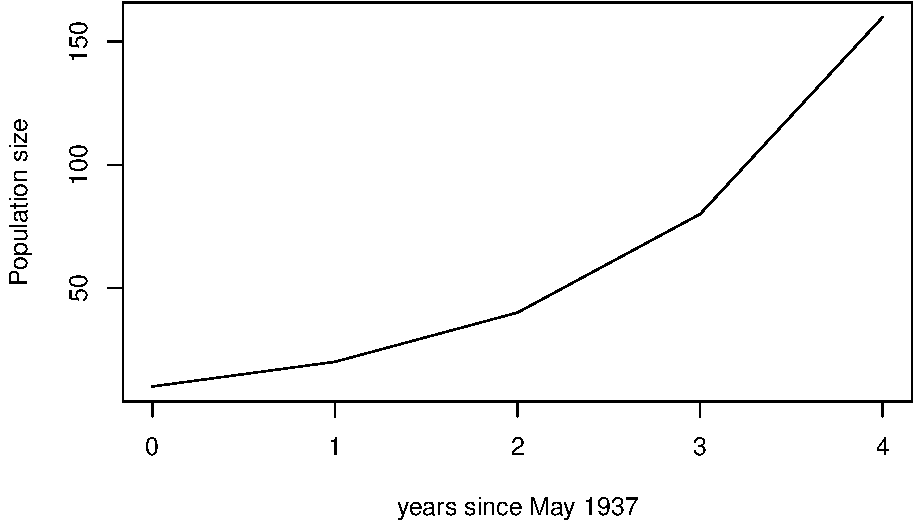
\includegraphics{BIOL-3295_files/figure-latex/unnamed-chunk-18-1.pdf}

If you already have an existing plot you can add new lines using
\texttt{lines()}. For example,

\begin{Shaded}
\begin{Highlighting}[]
\KeywordTok{plot}\NormalTok{(}\KeywordTok{seq}\NormalTok{(}\DecValTok{1}\NormalTok{,}\DecValTok{4}\NormalTok{), }\KeywordTok{c}\NormalTok{(}\DecValTok{1}\NormalTok{,}\DecValTok{3}\NormalTok{,}\DecValTok{4}\NormalTok{,}\DecValTok{2}\NormalTok{), }\DataTypeTok{ylab =} \StringTok{"y-axis"}\NormalTok{, }\DataTypeTok{xlab =} \StringTok{"x-axis"}\NormalTok{)}
\KeywordTok{lines}\NormalTok{(}\KeywordTok{seq}\NormalTok{(}\DecValTok{1}\NormalTok{,}\DecValTok{4}\NormalTok{), }\KeywordTok{seq}\NormalTok{(}\DecValTok{1}\NormalTok{,}\DecValTok{4}\NormalTok{))}
\end{Highlighting}
\end{Shaded}

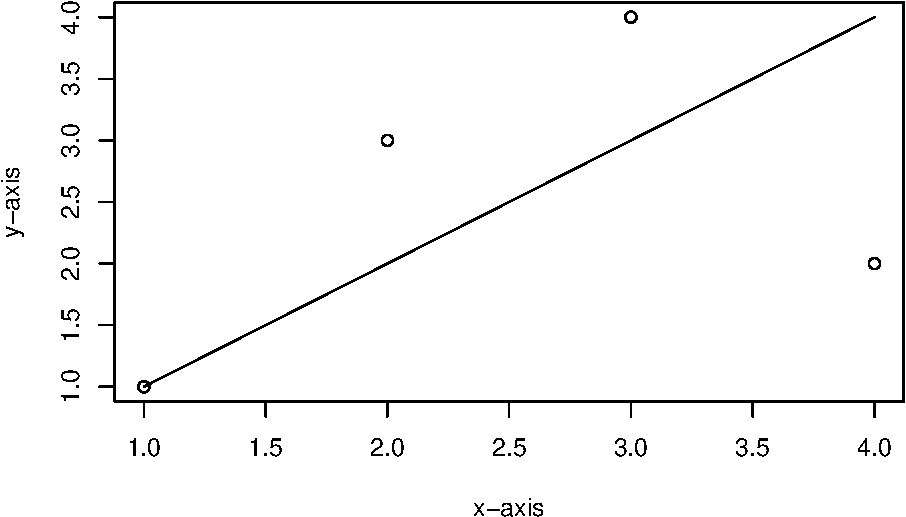
\includegraphics{BIOL-3295_files/figure-latex/unnamed-chunk-19-1.pdf}

 HAND IN

Write an R scipt that builds on the file you have previously made
\emph{protection-island.R}. Use the \texttt{lines()} command to add the
predicted population size assuming geometric growth using the commands
described in this section. If you have written the code correctly the
result should look something like this:

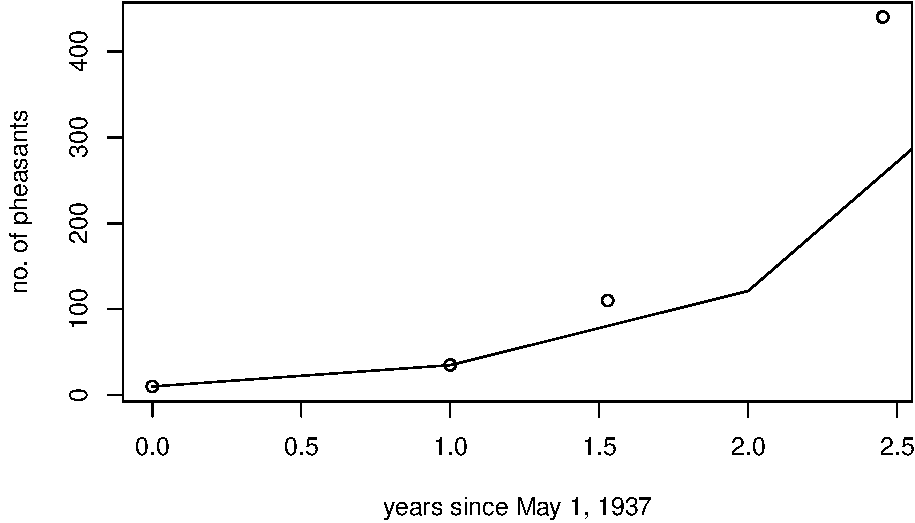
\includegraphics{BIOL-3295_files/figure-latex/unnamed-chunk-20-1.pdf}
You are to hand in your R Script. See \ref{RScript} for more
information. {[}10 marks{]}

\chapter{Fri Sept 25:{[}DRAFT{]} Doubling
times}\label{fri-sept-25draft-doubling-times}

\chapter{Tue Sept 29: {[}DRAFT{]} Density dependence and logistic
growth}\label{tue-sept-29-draft-density-dependence-and-logistic-growth}

\section{Required reading}\label{required-reading-2}

Vandermeer, J.H., Goldberg, D.E., 2013. Population Ecology: First
Principles (Second Edition). Princeton University Press, Princeton,
United States. p9-17.
\href{https://ebookcentral-proquest-com.qe2a-proxy.mun.ca/lib/mun/detail.action?docID=1205619}{Link}

\section{Questions}\label{questions-6}

\begin{enumerate}
\def\labelenumi{\arabic{enumi}.}
\item
  What is the equation for continous time logistic growth? Define all
  the symbols in the equation.
\item
  What does dN/dt mean?
\item
  Equibrium values
\end{enumerate}

\chapter{Thurs Oct 1: Solving the logistic growth equation using a
computer}\label{thurs-oct-1-solving-the-logistic-growth-equation-using-a-computer}

Numerical solutions to CT logistic growth

\chapter{Fri Oct 2: Data and the logistic
equation}\label{fri-oct-2-data-and-the-logistic-equation}

Density dependence + data

\section{Questions}\label{questions-7}

\begin{enumerate}
\def\labelenumi{\arabic{enumi}.}
\tightlist
\item
  Question 1.9 on p12 of Vandermeer and Gordon.
\item
  Question 1.10 on p12 of Vandermeer and Gordon.
\end{enumerate}

\chapter{Tues Oct 6: Discrete time models with density dependence using
a
computer}\label{tues-oct-6-discrete-time-models-with-density-dependence-using-a-computer}

\chapter{Thurs Oct 8: Solving the discrete time models with density
dependence using a
computer}\label{thurs-oct-8-solving-the-discrete-time-models-with-density-dependence-using-a-computer}

\chapter{Fri Oct 9: Analysis of discrete time
models}\label{fri-oct-9-analysis-of-discrete-time-models}

\chapter{Thurs Oct 15: Density-yield and density dependence in births
versus
deaths}\label{thurs-oct-15-density-yield-and-density-dependence-in-births-versus-deaths}

\chapter{Tues Oct 20: Balsam fir}\label{tues-oct-20-balsam-fir}

\chapter{Thurs Oct 22: Stage-structured
models}\label{thurs-oct-22-stage-structured-models}

\begin{itemize}
\tightlist
\item
  The idea of stage-structured models.
\item
  Multiplying matrices.
\item
  Eigenvalues of 2 x 2 matrix
\end{itemize}

\chapter{Fri Oct 23: Stage-structured
dynamics}\label{fri-oct-23-stage-structured-dynamics}

\begin{itemize}
\tightlist
\item
  Eigenvalues and eigenvectors
\item
  Diagrams
\end{itemize}

\chapter{Tues Oct 27: Yellow
columbine}\label{tues-oct-27-yellow-columbine}

\chapter{Thurs Oct 29-Fri Oct 30: Midterm {[}due Fri Nov 6 at
5pm{]}}\label{thurs-oct-29-fri-oct-30-midterm-due-fri-nov-6-at-5pm}

\chapter{Tues Nov 3: Evolutionary
ecology}\label{tues-nov-3-evolutionary-ecology}

\chapter{Thurs Nov 5: Evolutionary
ecology}\label{thurs-nov-5-evolutionary-ecology}

\chapter{Fri Nov 6: Evolutionary
ecology}\label{fri-nov-6-evolutionary-ecology}

\chapter{Tues Nov 10: Evolutionary
ecology}\label{tues-nov-10-evolutionary-ecology}

\chapter{Thurs Nov 12: Evolutionary
ecology}\label{thurs-nov-12-evolutionary-ecology}

\chapter{Fri Nov 13: Evolutionary
ecology}\label{fri-nov-13-evolutionary-ecology}

\chapter{Tues Nov 17: Evolutionary
ecology}\label{tues-nov-17-evolutionary-ecology}

\chapter{Thurs Nov 19: Evolutionary
ecology}\label{thurs-nov-19-evolutionary-ecology}

\chapter{Fri Nov 20: Evolutionary
ecology}\label{fri-nov-20-evolutionary-ecology}

\chapter{Final project ideas}\label{final-project-ideas}

{[}DRAFT{]}

For your final project you may choose either:

\begin{enumerate}
\def\labelenumi{\arabic{enumi}.}
\tightlist
\item
  Review paper: Read and synthesize information on a new topic in
  population and evolutionary ecology that we have not considered in
  class.
\end{enumerate}

or,

\begin{enumerate}
\def\labelenumi{\arabic{enumi}.}
\setcounter{enumi}{1}
\tightlist
\item
  Analysis: Download and visualize a dataset relevant to population and
  evolutionary ecology. Discuss your graphs in the context of a
  principle in population and evolutionary ecology.
\end{enumerate}

Use
\href{https://www-sciencedirect-com.qe2a-proxy.mun.ca/science/article/pii/0169534796100379?via\%3Dihub}{Dias
et al. 1996} \emph{Sources and sinks in population biology} as a guide
for what a final project that is a \emph{Review} should aspire to look
like.

If you choose to do a final project that is an \emph{Analysis} you
should use some of the exercises we have completed for class as a guide
(for example, the Doubling time, Protection Island, Yellow columbine, or
balsam fir analyses). Note that you will need to write your final
project as a report, rather than a series of questions.

Some examples of final project topics are:

Review paper: - Population dynamics in warming environments. -
Population dynamics in seasonal environments. - Spatial population
dynamics. - Metapopulations.

Analysis:

\section{How to read scientific
papers}\label{how-to-read-scientific-papers}

Please consult
\href{https://www.research4life.org/blog/how-to-read-a-scientific-paper/}{How
to Read a Scientific Paper (2014)} for the recommended approach to
`reading' journal articles. Steps 1,2, and 4 are good advice, but step 3
may not be relevant for some readings.

\section{Sources for datasets}\label{sources-for-datasets}

\section{Grading Rubric: Review}\label{grading-rubric-review}

\section{Grading Rubric: Analysis}\label{grading-rubric-analysis}

\backmatter

\end{document}
